%!TEX root = ../MasterThesis.tex

\chapter{Concept and Design of the System} % (fold)
\label{cha:design_system}

This main part of the Master thesis looks into the concept and design of a collaborative system that will improve the situation described in the scenario in Section~\ref{sec:scope_thesis}. Initially this chapter will discuss the overall concept of the proposed system on an high level without going to much into implementation specifics. This will answer the question of what the system is and should be able to achieve. After this initial conceptual view the chapter will further look into existing design approaches and discusses why they are of no use in this specific situation. Lastly a novel system design approach is proposed, which is based on Semantic Web and peer-to-peer communication technologies to improve the current situation, and support the investigation of E-commerce fraud incidents in an inter-institutional team.

% sub chapter design overview
%!TEX root = ../MasterThesis.tex

\section{Concept of System}
\label{sec:system_concept}

Based on the explanations in Chapter~\ref{cha:context_analysis}, and especially the scope definition for this Master thesis in Section~\ref{sec:scope_thesis}, the collaborative system for investigating \gls{E-commerce} fraud incidents have to answer the central question:\@

\begin{quotation}
  \textit{Is this really a valid \gls{E-commerce} transaction?}
\end{quotation}

The relevant stakeholders, that need to be involved in the investigation process, are:\@

\begin{enumerate}
    \item \textbf{merchant}, who can provide additional information of each \gls{E-commerce} transaction in question
    \item \textbf{\gls{PSP}/issuer}, that have information about the credit card usage patterns and the original credit card owner
    \item \textbf{\gls{LSP}}, who can offer information about whether the order has already been shipped or not, and in the former case to whom it has been handed over
\end{enumerate}

Ideally each of them would make parts of their internal data structures available for the other participants to access and query for. This would allow the stakeholder, who has to authorize or validate a suspecious credit card payment, to analyse all available information, as depicted in the Figure~\ref{fig:images_system_overview}.\@

\begin{figure}[H]
	\centering
		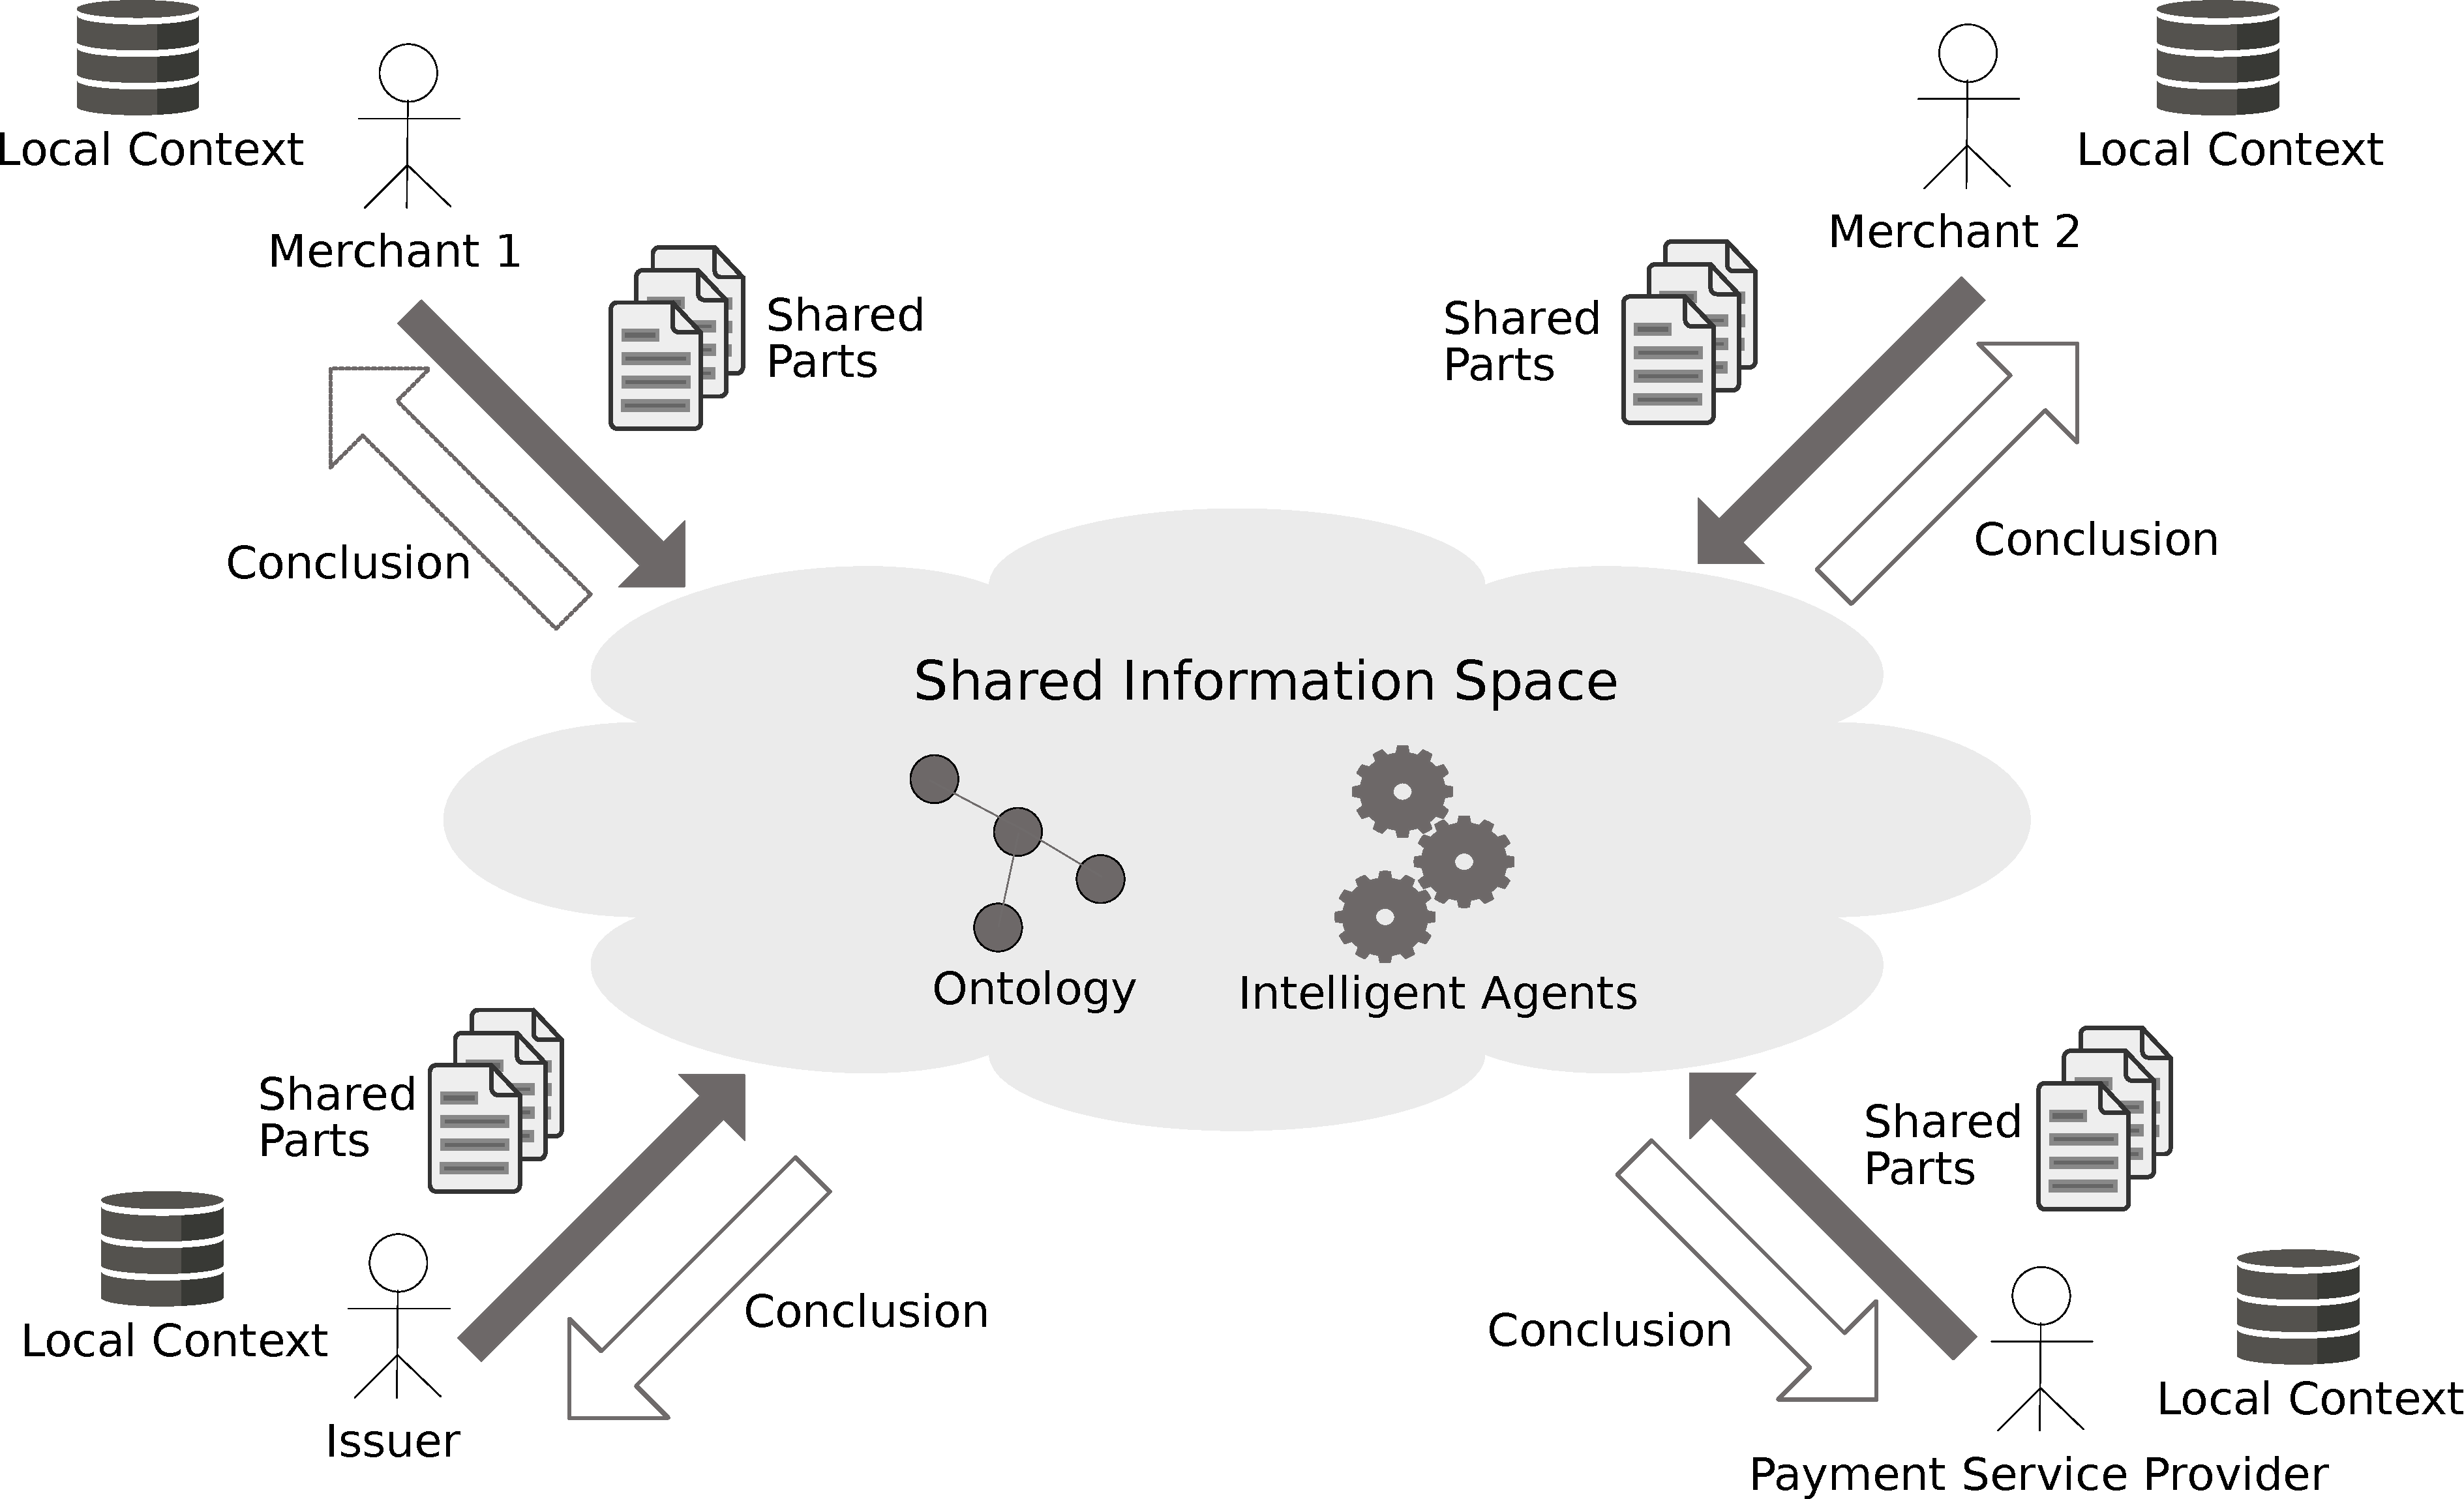
\includegraphics[width=0.9\columnwidth]{images/system_overview.pdf}
	\caption{High-level concept of the system}
\label{fig:images_system_overview}
\end{figure}

Due to the fact that data from various sources have to be combined into a shared understanding of the \gls{E-commerce} activities of a consumer, there is an urgent need to harmonize and transform the information into a shared data model. Based on the discussions in Chapter~\ref{cha:context_analysis}, and the analysis of the information each stakeholder holds and transmits to others, the following initial data relationships can be conducted for the \gls{E-commerce} scenario (see Figure~\ref{fig:images_data_model}). This figure shows not only the relevant information from the local contexts of each stakeholder, but also how they can be combined within a shared information space. \\

\begin{figure}[!ht]
  \centering
  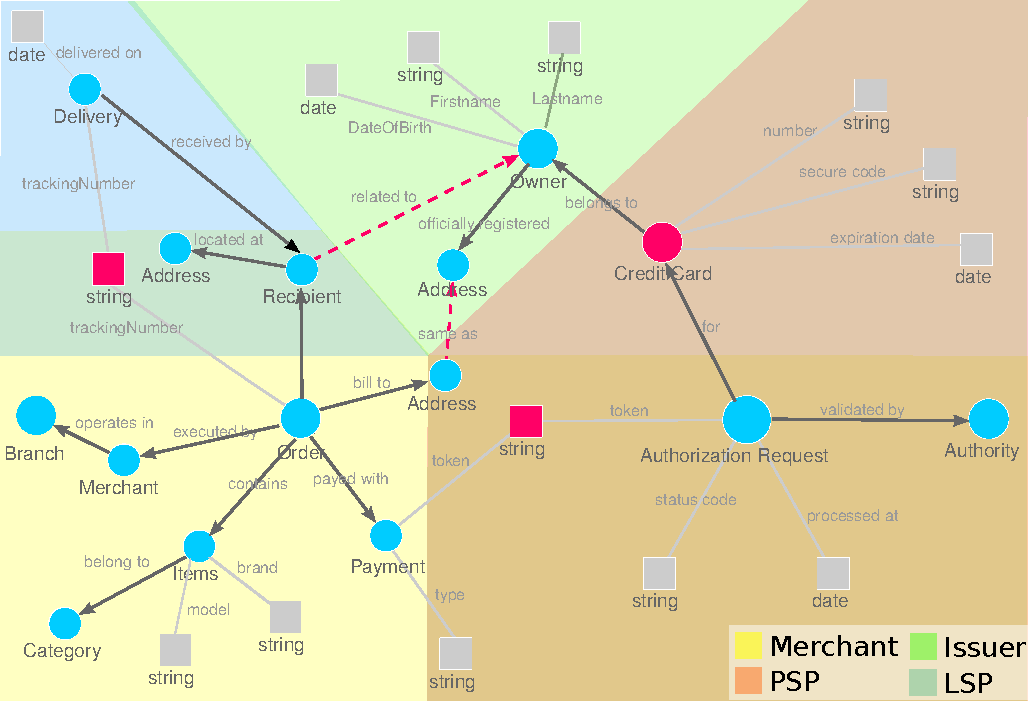
\includegraphics[width=0.9\columnwidth]{images/ontology_scenario_1.pdf}
  \caption{Data relations in the \gls{E-commerce} scenario\protect\footnotemark}
\label{fig:images_data_model}
\end{figure}

As one can see there are connection points between these stakeholders. Those can be used as a reference for joining the distributed information into a combined view of the \gls{E-commerce} order. There are actually three major connection points: \@

\begin{enumerate}
  \item \textbf{payment token}: shared between merchant and \gls{PSP}
  \item \textbf{tracking number}: shared between merchant and \gls{LSP}
  \item \textbf{credit card}: shared between issuer and \gls{PSP}
\end{enumerate}

In addition to these connection points one can also see the important validation points in the Figure~\ref{fig:images_data_model}. These are points that have an influence on the decision whether an \gls{E-commerce} transaction is evaluated as suspecious or not. The two main criterias are: \@

\begin{enumerate}
  \item \textbf{billing address}: the billing address of the order has to match the registered address of the owner of the credit card used
  \item \textbf{recipient}: the recipient of the delivery has to be related to the owner of the credit card
\end{enumerate}

\footnotetext{Legend: green: issuer, red: \gls{PSP}, yellow: merchant, blue: \gls{LSP}}

Whereas the first criteria can be examined during the authorization process of the credit card payment based on the information transmitted between merchant and \gls{PSP}, the second one is more difficult to validate (or can not be verified at all). The only check the \gls{LSP} is able to do before they are handing over the packaged items to the recipients, is to verify that they are the ones mentioned in the order. If they are somehow related to the owner of the credit card, or just a fraudster misusing the credit card data can not be confirmed at that point. \\

Also the merchants, the \gls{PSP}s and issuers have no clue. Whereas the merchants are able to validate whether a consumer has send items to that shipping address before, they can not restrict a consumer to choose only validated recipient addresses for shipping the order. Doing so will have a negative impact on the business success of the online merchant. The \gls{PSP}s and issuers can not analyze this fact either, as both participants will not receive the information about the delivery address of an order with the credit card authorization request coming from a merchant. \\

But just sharing the fact whether the shipping and billing address of an order is different between the relevant stakeholders is not enough. Although this information is necessary, it is not sufficient to make a decision about suspecious transactions. Other necessary information are whether the consumer has send orders to this shipping address before, and the information about the content of the current order. Nevertheless, as mentioned in Section~\ref{sec:scope_thesis} looking at just a single transaction of one of the merchants is still not enough to solve the \gls{E-commerce} fraud scenario, that this thesis examines. \\

Therefore the idea is to combine the transaction information from various merchants, \gls{LSP}s, \gls{PSP}s and issuers into one large, combined and shared information space to be able to analyze if there are any orders that look extraordinary, and are likely not being made by the owner of the credit card to a certain extend. One can already see that the proposed solution will have to deal with statistical evaluations and probabilities. Starting with the credit card in question the issuers can query for the order details of transactions, that have been done recently with the credit card online. For that they will likely have to query the \gls{PSP}s for the payment tokens first, before asking the merchants for order details to any of those payment tokens. At the end each online transaction can be mapped into a schema like the one shown in Figure~\ref{fig:images_data_model}, building up a large graph of entities and  the relationship between them, having the specific credit card in the center of it. An abbreviated sample graph of this procedure can be seen in Figure~\ref{fig:images_credit_card_graph}. \\

One can clearly recognize the different clusters of transactions by merchant. Still this first collection of the various order information into one large data set is just the beginning of the analysis. Based on the information received the issuer can already filter out transactions, that have been shipped to different addresses than the one the credit card owner is registered for. Especially for those cases it might be worth to ask for additional information from the affected merchants to figure out if the consumer has used these shipping addresses before. As a result the existing graph can be further enriched with suplementary transactional information from merchants at any time if needed. In addition to the address information the issuer can also analyse the item information (incl.\ category, brand and model) of each order. \\

\begin{figure}[!ht]
  \centering
  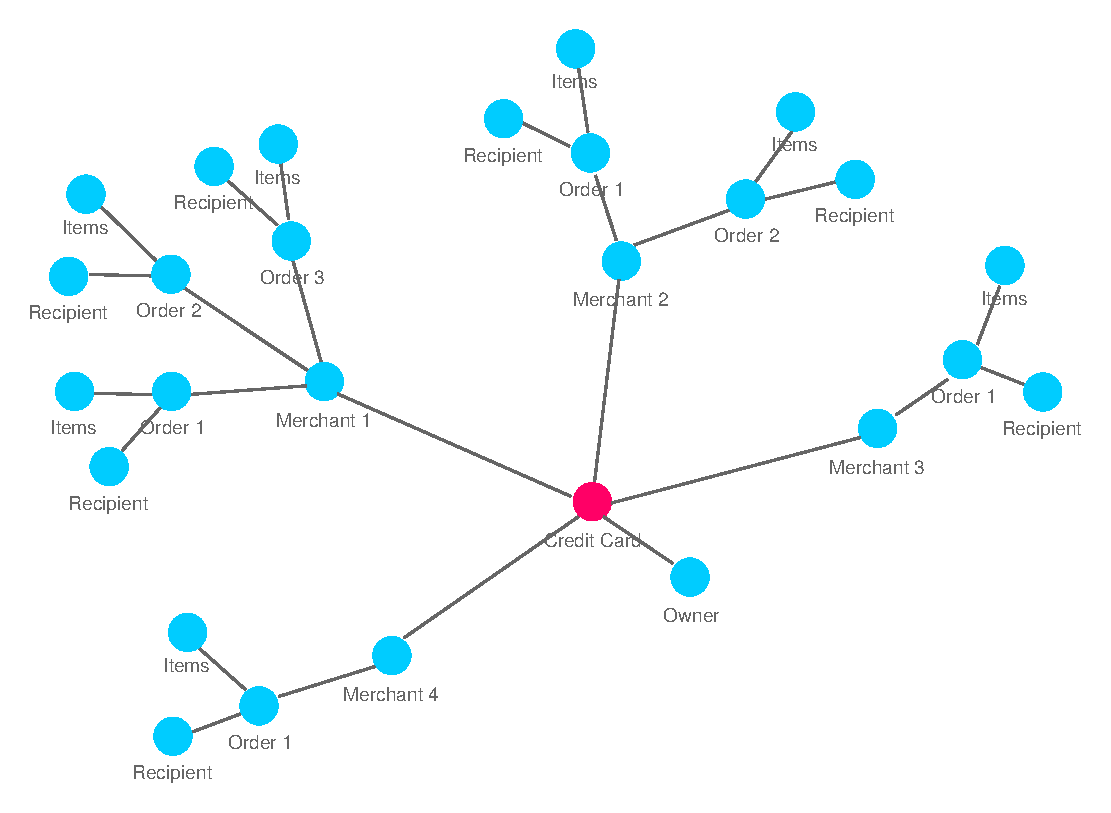
\includegraphics[width=0.9\columnwidth]{images/ontology_scenario_2.pdf}
  \caption{Clusters of E-commerce transactions by merchant}
\label{fig:images_credit_card_graph}
\end{figure}

But as said before, analysing the cluster of transactions from each merchant \textbf{\underline{alone}} will not be sufficient to come up with a solid decision about a suspecious transaction. This is mostly due to the usage pattern of the fraudsters, that have been described in the scenario selected for this Master thesis in Section~\ref{sec:scope_thesis}. Due to this scenario the various order details from the merchants have to be mapped against each other, so that the initial graph can be easily transformed into complementary representations, whose uses different criterias to cluster the transactions --- such as recipient addresses, branches of the merchants, or product-related information. This reshaping of the graph can lead to new insights about the ``normal'' shopping behaviour of the original credit card owner, and can make deviations from this behaviour visible. Visualizing the graph data as a clustered graph on screen supports the explorative nature of knowledge generation and perception, and can help speed up the investigation of the \gls{E-commerce} fraud incidents. An example visualization of a clustered graph is shown in Figure~\ref{fig:images_graph_viz}. \\

\begin{figure}[!ht]
  \centering
  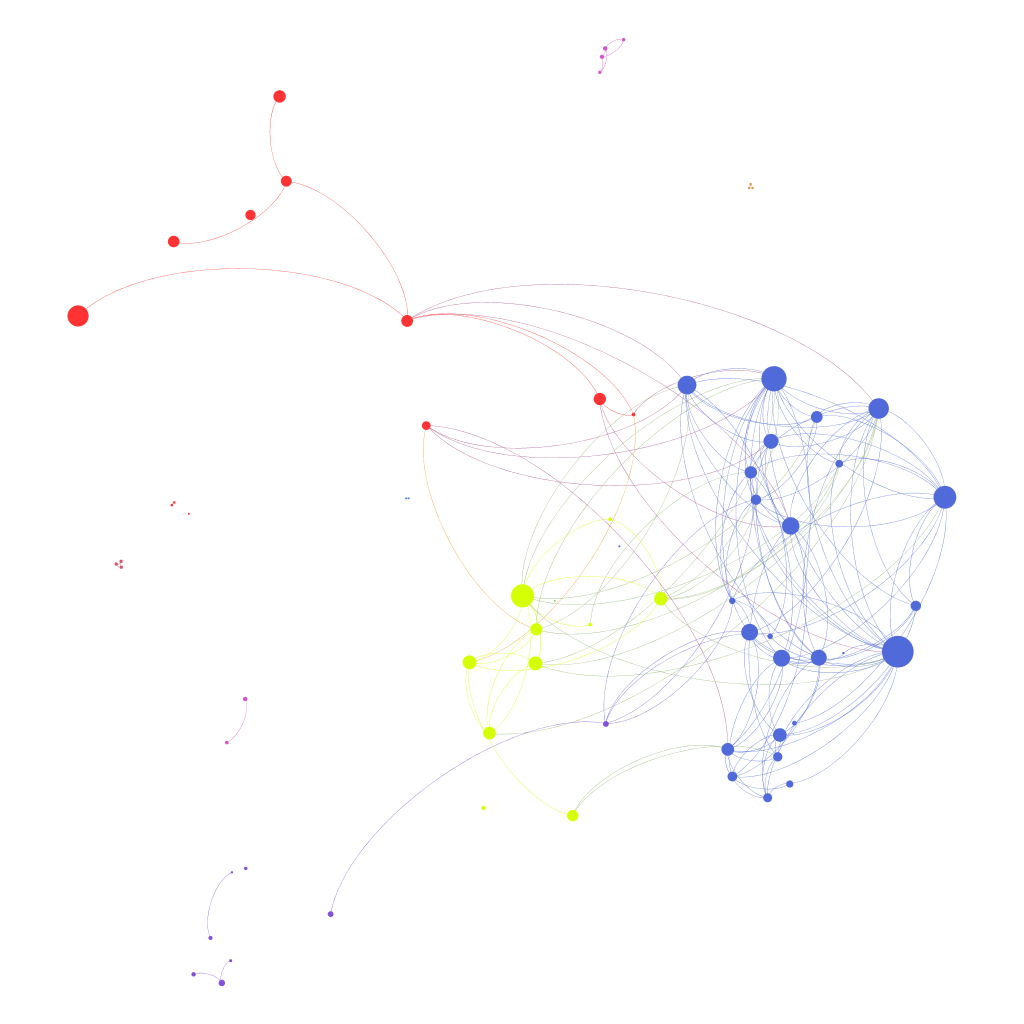
\includegraphics[width=0.9\columnwidth]{images/GraphViz.png}
  \caption{An example visualization of a clustered graph \citep{visjsshowcase}}
\label{fig:images_graph_viz}
\end{figure}

 In addition to these clustered graphs the system can also support the investigation of the incidents by changing the type of visualization used based on the criteria chosen for the clustering of the order details; e.g.\ when clustering them based on location information such as the shipping addresses the system can present the information as a heat map on a chart such as displayed in Figure~\ref{fig:images_map_heatmap}. \@

\begin{figure}[H]
  \centering
  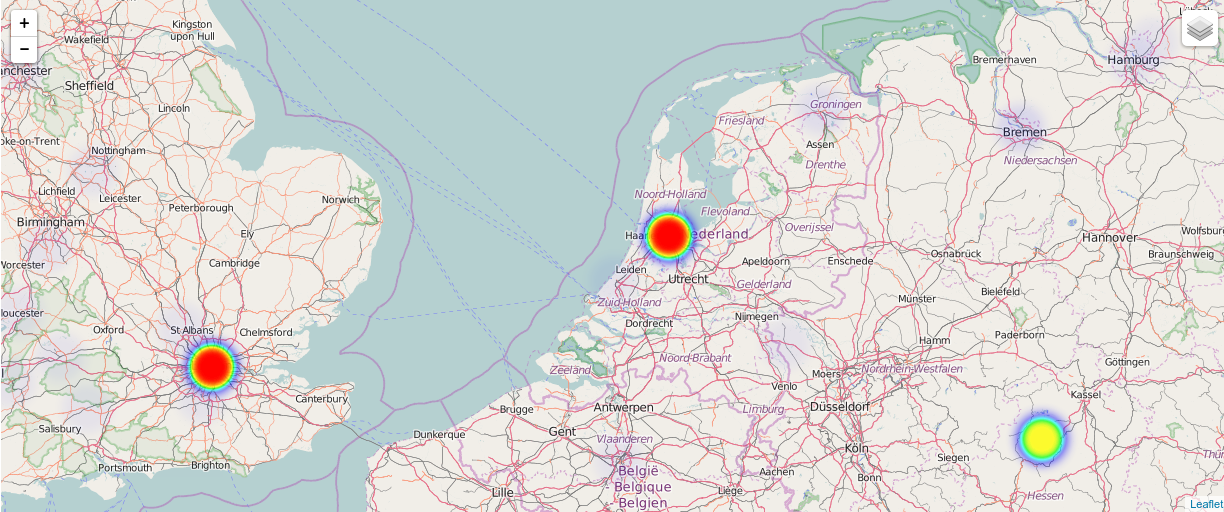
\includegraphics[width=0.9\columnwidth]{images/Heatmap.png}
  \caption{Heatmap displaying clusters of location-based information}
\label{fig:images_map_heatmap}
\end{figure}

To conclude the system have to support the collection and combination of \gls{E-commerce} transaction information from various sources into a large clustered graph, that can be analysed from multiple view points to validate, if there is any transaction that stands out from the ``normal'' shopping behaviour of the original credit card owner. The starting point is a sequence of recent credit card activities, that the issuer can provide to the other participants. The initial graph will collect and cluster the information from each merchant based on this list. In case there are suspecious information in one of the clusters of the merchant, the issuer can ask for further details and enrich that specific cluster with additional order details for this customer and that merchant. In the final step the system has to do the mapping of the order detail information between each merchant to allow subsequent analysing and clustering of the transactions.

% section system_overview (end)


% sub chapter existing approaches
%!TEX root = ../MasterThesis.tex

\section{Existing System Design Approaches}
\label{sec:system_approaches}

When trying to solve issues of information integration between organisations there are already existing solutions, that have to be examined whether they might fit the E-commerce fraud investigation scenario or not.

\subsection{The \gls{ETL} processes}
\label{subsec:etl_process}

To begin with, retrieving, transforming and combining data from multiple dispersed data sources is not a completely new problem and is actually part of an ``Extract-Transform-Load'' or \gls{ETL} process within an organisation. The basic idea is the same as the concept shown in this thesis; namely to get as much information as possible from the various databases, that are in use within a company, harmonize (aka transform) the information from each of them into a shared data model, and use the cleaned up and combined information repository for doing advanced business analytics and predictions. The whole process is visualized in Figure~\ref{fig:images_etl_process}. \\

\begin{figure}[!ht]
  \centering
  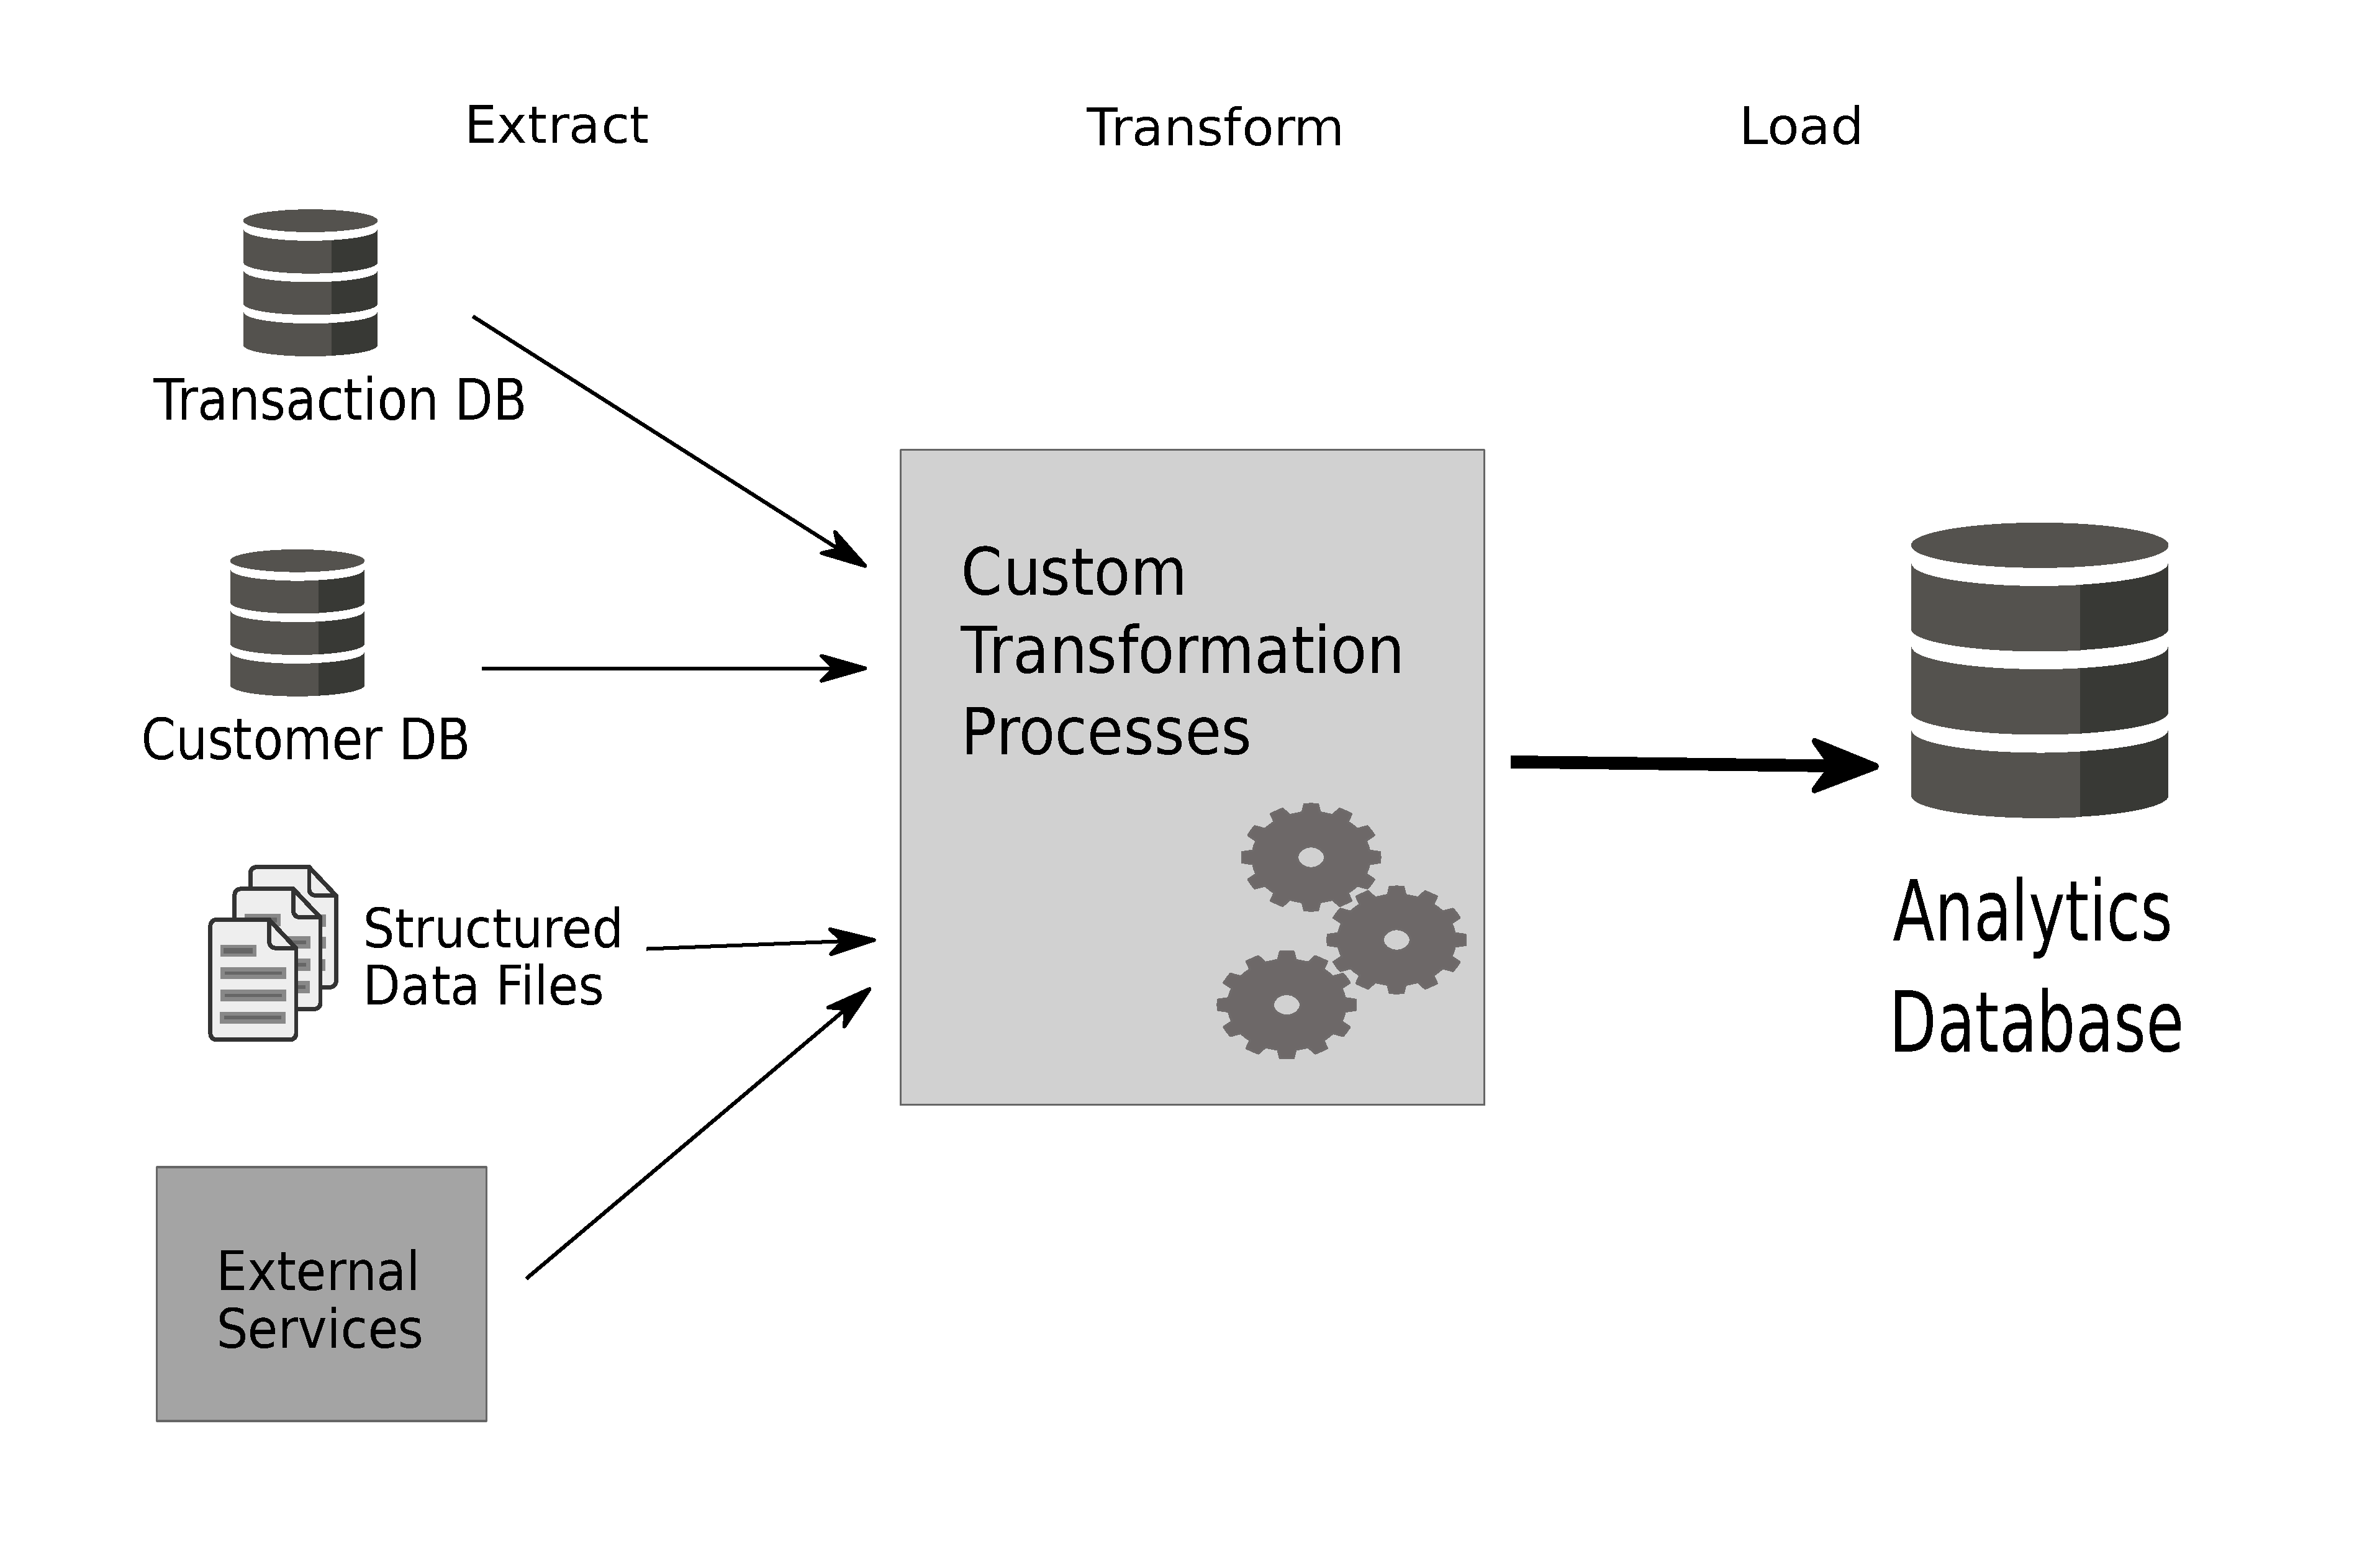
\includegraphics[width=0.7\columnwidth]{images/etl_process.pdf}
  \caption{\gls{ETL} process within a company \citep[pg. 165]{wood2014linked}}
\label{fig:images_etl_process}
\end{figure}

Still these processes rely on an in-depth knowledge of the data structures, that are used in each of the information sources as well as direct access to the databases and files for information retrieval. Although these conditions are not cumbersome to work with within an organisation, they will be a real show stopper if one has to integrate data sources across company boundaries. As the integration in the \gls{ETL} processes takes place on the database level, allowing external access to your databases will not only open up access to your business internals, but will also make it more complicated to change the underlying database structure and software. Any changes to one of these require a negotiation between the owner of the data source and all of the partners attached to it. \\

Beside this limited usage for the E-commerce fraud investigation scenario at the whole, one can assume that these processes are still in use for the daily business of each stakeholder. They can be helpful at a later point in the discussion about how a stakeholder can prepare and transform his internal data resources for external consumptions.

% section etl_process

\subsection{Web of Services}
\label{subsec:web_services}

With the development of the E-commerce scenario there was also a need to integrate business functionality from various service providers operating on the Internet. Good examples for this are the integration of the \gls{PSP} into the payment as well as the \gls{LSP} for the shipping process. These approaches resulted in the ``Service Oriented Architecture'' paradigm, that enables application services provided by different vendors to talk to each other via a public facing programming interface (aka \gls{API}). The only requirement for such interoperability to work properly is, that each public interface follows some standardised or commonly agreed upon guidelines to be vendor-, platform- as well as language-agnostic. One possible implementation of these concepts are the so-called Web Services, that use the WS* protocols and standards from the \gls{W3C} with the extensible markup language (aka \gls{XML}) and the \gls{HTTP} protocol at their core \citep{josuttis2007soa}. \\

Like the \gls{HTML} format, that is used to represent Web pages on the Internet, \gls{XML} is originally based on \gls{SGML}, but instead of formalising markup tags for structuring and styling textual content it is a meta-language allowing everyone to define his or her own markup languages. In this matter it doesn’t dictate what tags are available to structure the information; instead it includes some basic guidelines for creating wellformed and valid documents that uses domain-specific tags, which can be freely defined and structured by the creator of the XML document. Therefore it is better suited in situations where a computer has to parse and evaluate the content of a message (assuming the computer program knows the structure of the message) \\

In an additional step the author of the API could also specify an XML schema for each message, which describes the structure of the message with all the possible elements, their ordering, nesting level and data types in detail. By doing so the XML parser program can later verify the content of a retrieved message against the XML schema and check if it is a valid document (related to the schema definition). XML schematas are also expressed in XML format and have been standardised by the W3C. Being able to create custom markup languages via XML has a huge benefit for machine-to-machine communication and is the basis for integrating Web Services (via the WS* protocols), but it still has limitations when it comes to figure out the semantics of those XML messages. This is mostly due to the fact that each XML document represents a new markup language and needs a specific XML parser to be understood by the machine; also to distinguish commonly used tag names in an XML document the creator has to place them into specific namespaces (aka XML namespaces). But those XML namespaces further complicate the automatic processing of XML documents and increases the necessity to have custom instances of XML parsers for each XML document \citep{taylor2008p2p}. \\

Mapping the scenario onto the Web of Services approach would mean, that each merchant has to provide a specific \gls{HTTP} \gls{API} endpoint for querying transaction information by the issuer or \gls{PSP}. Additionally each issuer or \gls{PSP} has to collect all available information from the affected merchants (based on recent credit card authorization requests) and combine these various transactional data locally to be able to make an analysis of them that might lead to a decision regarding the E-commerce fraud question from above. \\

This will also mean that each merchant has to provide a separate entrypoint for issuers and \gls{PSP}s to give access to selected information from the internal backend databases. These endpoints have to make safe and secure, so that only allowed parties can access these records. In addition the information from the various internal databases of the merchants have to be converted into a format suitable for external consumption --- in this case a structured \gls{XML} file. \\

Issuers and \gls{PSP}s on the other hand have to maintain a list of \gls{HTTP} \gls{API} endpoints and their respective credentials to access the data from each merchant. Additionally they will have to provide a mapping of each merchant's specific data from the \gls{XML} file to the internal analytics database of the issuer or \gls{PSP}. They also have to trigger internal backend services in case of a suspecious E-commerce transaction that will query the \gls{HTTP} \gls{API} endpoint of the corresponding merchant for further information. \\

As conclusion one could easily see that there are huge efforts on all participating parties to provide information to or integrate data from each other. As there is no common way to access the information at the merchant side (beside the lower level HTTP protocol and XML data format), there have to be a lot of collaboration between each combination of stakeholders for deciding on access patterns and needed data structures in the beginning. Most importantly as each \gls{HTTP} \gls{API} endpoint will be publicly accessible via the Internet it will also opens up a new opportunity for hackers to get access to personal or payment related information.

% subsection web_services (end)

\subsection{Web of Data}
\label{subsec:web_data}

``The Web is full of intelligent applications, with new innovations coming every day'' \citep{allemang2011semantic}. But each of those intelligent Web applications is driven by the data available to them. Data that is likely coming from different places in the global information space — accessible usually via a custom API on the server hosting those resources (see Section~\ref{subsec:web_services}). The more consistent the data available to the smart Web application is the better the service and its result will be. But to support an integration of the data from various Web services the semantics of the information delivered by each service has to be available — and there has to be a generalised, formalised way to express the semantic of that data. The focus on a standard that allows Web services to express the semantics of the data they provide also allows for global scalability, openness and decentralisation, which are the key principles of the World-Wide Web. The Semantic Web tries to give a solution for this problem by providing the Resource Description Framework (aka \gls{RDF}) and related technologies (e.g. RDF schema, SPARQL, OWL, \ldots) for describing, linking and querying the data that a Web service delivers. But it doesn’t reinvent the wheel; instead the Semantic Web builds upon existing, proven technologies like XML, XML namespaces, XML schemata and the \gls{URI} to uniquely address resources on the Web \citep{allemang2011semantic}. \\

A huge benefit of the Web of Data approach is, that the resources delivered are self-describing. They do not only have a consitent and meaningful syntax, but are also semantically self-contained. As of this each merchant has to provide a semantically description of the resources used in a transaction in a standard way --- e.g.\ by using \gls{W3C} standards like \gls{RDF}, \gls{RDFa} or \gls{JSON-LD}. Each merchant also have to provide a \gls{HTTP} \gls{API} endpoint to access and query for the resources, utilizing a query language like \gls{SPARQL}. \\

Each issuer or \gls{PSP} can access these \gls{HTTP} \gls{API} endpoints with her credentials and query for specific information from the public ``information database'' from a merchant. The results of each query can be easily combined into an existing database based on the merging capabilities of \gls{RDF}. The resulting analytic database can be used by the issuer or \gls{PSP} to run queries against or use them with intelligent reasoning tools from the Semantic Web standards for investigation of an E-commerce transaction. \\

The resulting issues and problem are mostly the same as with the Web of Services approach --- beside that the Web of Data offer an unique and integrated way to describe the structure and semantic of the data received from another party. The initial efforts for the implementation of this scenario is also quite high, even if it is lower than with the Web of Services approach. This is mostly due to the fact that there are already some industry-wide and commonly agreed upon ontologies and taxonomies, that are able to describe most of the resources in an E-commerce transaction (e.g.\ GoodRelations Ontology, Schema.org). As it is more likely that merchants do already use them to encode at least some of the data in their backend databases for machine-to-machine communication, it will also descrease the effort on merchant side to provide them for the issuers and \gls{PSP}s. Still these parties have to define the kind of queries and reasoners that might be useful to investigate an E-commerce transaction with the objective to figure out if it is fraudulent or not and have to implement them into their own backend systems.

% subsection web_data (end)

% section system_approaches (end)


% sub chapter design proposal
%!TEX root = ../MasterThesis.tex

\section{System Design Proposal}
\label{sec:design_proposal}

As the previous section showed, existing approaches are of limited use for the design of a collaborative system to support the \gls{E-commerce} fraud investigation scenario described in Section~\ref{sec:scope_thesis}. The leading approach for such a system will have to combine the best characteristics from the Web Service and the Semantic Web designs. \\

As for the Web Service approach, the most valuable aspects of it are: \@

\begin{itemize}
	\item access to the \gls{HTTP} endpoints can be limited to a certain set of communication partners
	\item these partners have to authenticate with each Web Service first
	\item based on the identification of the partners only certain parts of information can be returned, and execution of operations can be restricted
\end{itemize}

Looking at the Semantic Web approach, it's most interesting functionalities are: \@

\begin{itemize}
	\item providing information in a semantically self-contained way
	\item the ability to merge information from different \gls{RDF} data stores
	\item the graph-based data model underlying the \gls{RDF} data stores
	\item the usage of \gls{SPARQL} to query and analyze the locally combined data sets
\end{itemize}

In the following section the thesis will come up with an approach that uses the fundamental technologies from the Semantic Web for information sharing and integration as well as peer-to-peer communication technologies for securing and restricting access to the \gls{RDF} data sets from the relevant participants of the \gls{E-commerce} fraud investigation scenario. It will start with a discussion of the semantics of the underlying \gls{RDF} files and how these can be combined across various organizations. After that it shows how these information can be provided to the relevant parties in the investigation scenario. It will continue with a detailed look into the partially centralized \gls{P2P} communication architecture and how that can be used for the proposed solution.

\subsection{Vocabulary alignment}
\label{subsec:vocab_align}

Although the \gls{RDF} format has build-in support for merging information from different data sources, this functionality is only working as expected if the ``triples'' in the dispersed data stores are using the same \gls{URI}s to refer to the same subjects or objects. In that case merging the ``triples'' from different \gls{RDF} data files will result in a local graph holding the combined information as shown in Figure~\ref{fig:images_combine_rdf_graph}. \\

\begin{figure}[!ht]
	\centering
		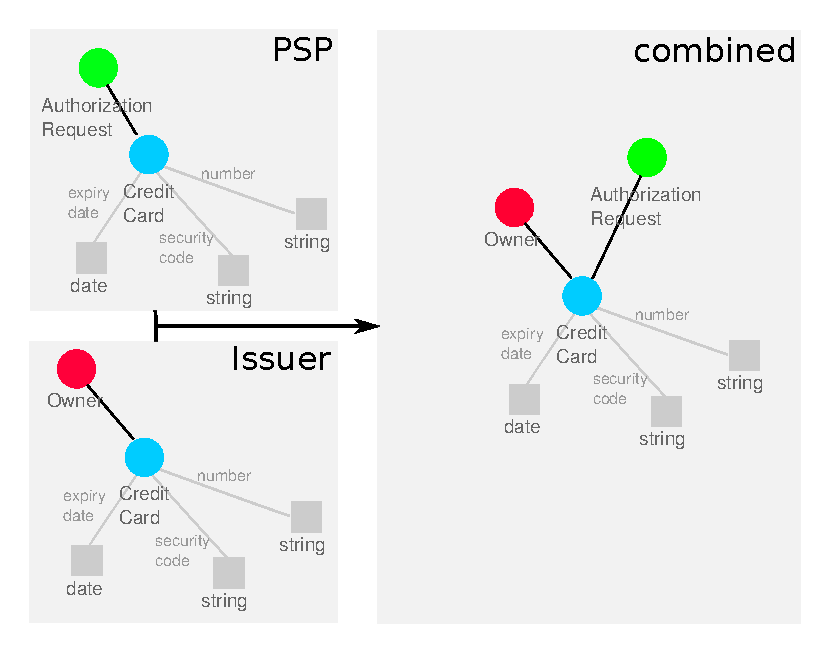
\includegraphics[width=0.9\columnwidth]{images/combine_rdf_graph.pdf}
	\caption{Combining two \gls{RDF} files containing the same credit card entity}
\label{fig:images_combine_rdf_graph}
\end{figure}

As a major objective of the \gls{E-commerce} fraud investigation system is to bring the various transactional information from online merchants, \gls{PSP}s and issuers together, combine them all and analyze the resulting graph from different viewpoints, the information exchanged between the relevant participants have to follow a common schema. A possible approach is to define a completely new schema for the proposed system and share it with every possible stakeholder. This schema will define all the entities and relations known to the collaborative system and would be expressed in \gls{RDFS} format. A major drawback of this approach is, that new partners of the system will have to do the conversion of their internal data structures to an \gls{RDF} file, that is compatible with the specific schema definition, before being able to participate in it. \\

Therefore a better approach is to take a look into commonly used \gls{RDF} schemata and vocabularies, and try to figure out if they can be used for describing the information, that need to be exchanged between participants of the \gls{E-commerce} fraud investigation system. When consulting the Semantic Web community for commonly agreed upon and highly referenced \gls{RDF} schema definitions, one will come up with this list (see Table~\ref{tab:used_vocab_rdf}):\@

\begin{table}[H]
\centering
\begin{tabular}{p{3cm}llp{4.5cm}}
\hline
\textbf{Name} & \textbf{Prefix} & \textbf{Describes} & \textbf{Namespace URI} \\
\hline
Dublin Core & dc: & Meta data & \url{http://purl.org/dc/terms/} \\
\hline
FOAF & foaf: & People & \url{http://xmlns.com/foaf/0.1/} \\
\hline
Geo & pos: & Positions & \url{http://www.w3.org/2003/01/geo/wgs84\_pos\#} \\
\hline
Geo Names & gn: & Locations & \url{http://www.geonames.org/ontology\#} \\
\hline
Good Relations & gr: & Products & \url{http://purl.org/goodrelations/v1\#} \\
\hline
RDF & rdf: & Core framework & \url{http://www.w3.org/1999/02/22-rdf-syntax-ns\#} \\
\hline
RDFS & rdfs: & RDF vocabularies & \url{http://www.w3.org/2000/01/rdf-schema\#} \\
\hline
Schema.org & schema: & Schema.org vocabularies & \url{http://schema.org/} \\
\hline
SKOS & skos: & Controlled vocabularies & \url{http://www.w3.org/2004/02/skos/core\#} \\
\hline
vCard & vcard: & Business Cards & \url{http://www.w3.org/2006/vcard/ns\#} \\
\hline
Web Ontology Language & owl: & Ontologies & \url{http://www.w3.org/2002/07/owl\#} \\
\hline
XML Schema Datatypes & xsd: & Data types & \url{http://www.w3.org/2001/XMLSchema\#} \\
\hline
\end{tabular}
\caption[Commonly used \gls{RDF} vocabularies on the Web]{Commonly used \gls{RDF} vocabularies on the Web \citep[pg. 41]{wood2014linked}}
\label{tab:used_vocab_rdf}
\end{table}

Based on these schema specifications describing a fictive consumer named ``Max Mustermann'' incl.\ his home address can be done by combining data utilizing the \gls{FOAF} and \gls{vCard} namespaces in a \gls{RDF} file, such as described in Listing~\ref{lst:sample_customer_mustermann} and visualized as graph in Figure~\ref{fig:images_sample_customer}. \@

\begin{listing}[H]
  \inputminted[linenos,
               numbersep=5pt,
               breaklines=true,
               frame=lines]{TURTLE}
               {./samples/sample_customer_mustermann.ttl}
  \caption{Personal related information about a fictive consumer in \gls{RDF}}
\label{lst:sample_customer_mustermann}
\end{listing}

\begin{figure}[H]
	\centering
		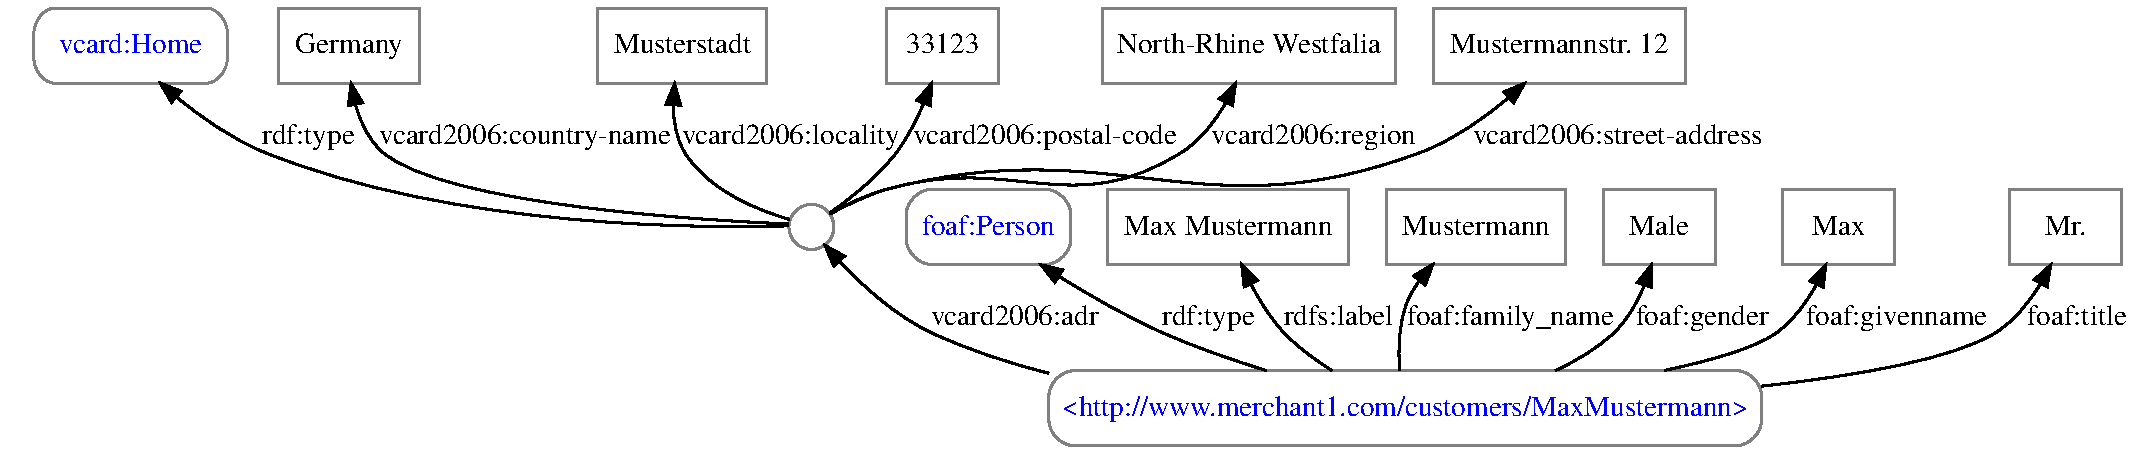
\includegraphics[width=\columnwidth]{images/sample_customer_mustermann.pdf}
	\caption{Graph representation of consumer information from Listing~\ref{lst:sample_customer_mustermann}}
\label{fig:images_sample_customer}
\end{figure}

Looking back to the initial data model from Section~\ref{sec:system_concept} one can map the information, that are currently available in the \gls{E-commerce} scenario, to the existing \gls{RDF} vocabularies such as follows (see Table~\ref{tab:map_tx_rdf_vocab}):\@

\begin{table}[H]
\centering
\begin{tabular}{p{5cm}l}
\hline
\textbf{Information} & \textbf{RDF vocabulary} \\
\hline
Consumer & FOAF \\
\hline
Credit Card Owner & FOAF \\
\hline
Billing Address & vCard \\
\hline
Shipping Address & vCard \\
\hline
Location Information & Geo Names \\
\hline
Merchant & GoodRelations \\
\hline
Items & GoodRelations \\
\hline
Item Categories & GoodRelations \\
\hline
Brands & GoodRelations \\
\hline
Payment Types & GoodRelations \\
\hline
\end{tabular}
\caption{Possible usage of \gls{RDF} vocabularies for \gls{E-commerce} transaction information}
\label{tab:map_tx_rdf_vocab}
\end{table}

As this table shows there are some parts of the \gls{E-commerce} data model that can be expressed with existing \gls{RDF} vocabularies extensively --- such as personal related information via \gls{FOAF} and \gls{vCard}, whereas other parts can not be stated in-depth (e.g. credit card information), or are not specified at all (e.g.\ tracking of the delivery). Additionally some of the vocabularies are no longer actively maintained, such as GoodRelations. Due to these circumstances one usually have to build an own ontology that fills in the missing pieces and refers to the existing concepts whenever appropriate. Trying to model the information of a credit card as displayed in Figure~\ref{fig:images_data_model} will result in the \gls{RDFS} specification shown in Listing~\ref{lst:credit_card_vocab}. \@

\begin{listing}[H]
  \inputminted[linenos,
               numbersep=5pt,
               breaklines=true,
               frame=lines]{TURTLE}
               {./samples/vocab_credit_card.ttl}
  \caption{A specification for a credit card in \gls{RDFS}}
\label{lst:credit_card_vocab}
\end{listing}

But building a new ontology for handling the \gls{E-commerce} fraud investigation process is not the best approach. The result would be that participants have to access, understand and implement the desired \gls{RDF} data schema first, before they can share their information in the collaborative system. Looking back at the list of existing ontologies and vocabularies, that are actively used on the Web today, one will find the Schema.org vocabulary definition \citep{Schema.org}. This vocabulary was initially designed by the leading search engines (aka Google, Microsoft and Yahoo!) to allow authors of Web sites to markup their \gls{HTML} documents in a way, that they are better understood by those search engines (aka \gls{SEO}). The Schema.org vocabulary is actively maintained by its community, includes new concepts with each release and also offers an extension mechanism to implement additional vocabularies that are not part of the core specification \citep{SchemaExtensions}. In one of the past releases of the Schema.org core specification it also included all of the existing concepts of the GoodRelation ontology \citep{SchemaGoodRelation}. \\

As the merchants will provide semantic meta data for their products to improve their listing on search engine results (aka \gls{SEO}) in the vocabulary of Schema.org already, one can re-use parts of these information for the \gls{E-commerce} fraud investigation. Additionally, the wide-ranging scope of aspects that Schema.org declares make it a good fit to the \gls{E-commerce} fraud investigation scenario. Trying to map the initial data model from Section~\ref{sec:system_concept} to the Schema.org core specification will result in a data schema as displayed in Figure~\ref{fig:images_schema_org}. \@

\begin{figure}[!ht]
	\centering
		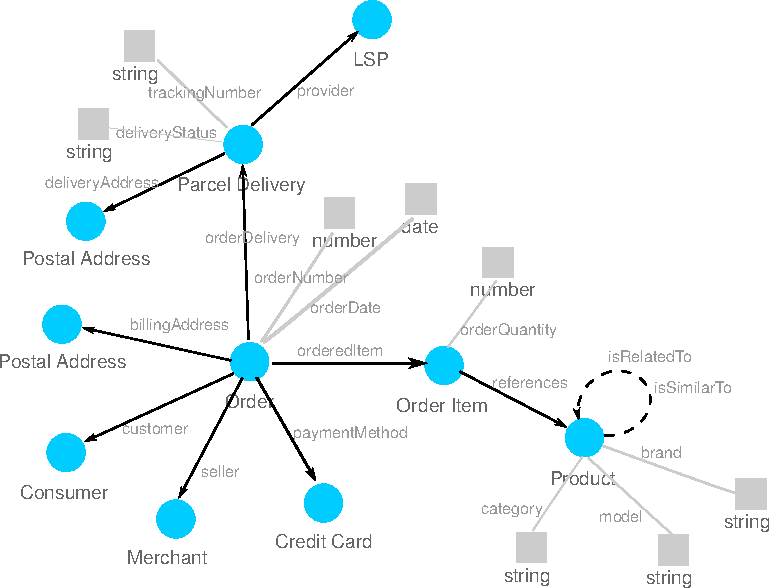
\includegraphics[width=0.8\columnwidth]{images/schema_org_mapping.pdf}
	\caption{Schema.org based mapping of an \gls{E-commerce} transaction}
\label{fig:images_schema_org}
\end{figure}

% subsec vocab_align

\subsection{Communication protocols}
\label{subsec:comm_protocol}

 The data is likely encoded in Microdata, \gls{RDFa} or \gls{JSON-LD}. \\

For the communication the \gls{WebRTC} is a good approach as it integrates well with existing enterprise IT infrastructures.
\\

\ldots

% subsec comm_protocol

\subsection{Using a partially centralized \gls{P2P} system}
\label{subsec:p2p_partially_centralized_system}

For the \gls{E-commerce} fraud scenario, that has been selected for this thesis in Section~\ref{sec:thesis_scope}, one can say that the issuer of a credit card is the party who initiates the collaborative fraud investigation. They are recognizing the active use (and likely misuse) of a credit card in the online and the offline world first, and are also getting a notification about any suspicious transactions made with it from their fraud prevention systems. Due to this fact, one can come up with a partially centralized \gls{P2P} architecture for the \gls{E-commerce} fraud investigation system, in that the issuer of a card in at the center and acts as a trusted party in this system. This issuer will initiate a collaborative session with the other required stakeholders based on the usage history of the credit card in question. During this \gls{P2P} communication session the merchants, \gls{PSP}s and \gls{LSP}s will share the required information with the issuer. In this process the data from the other stakeholders will be replicated to the issuer, who will build up a networked graph based on the Schema.org specification. So the main work will be on the issuer's side, who is the major driving party in the system, as depicted in Figure~\ref{fig:images_p2p_centralized}.\@

\begin{figure}[H]
	\centering
		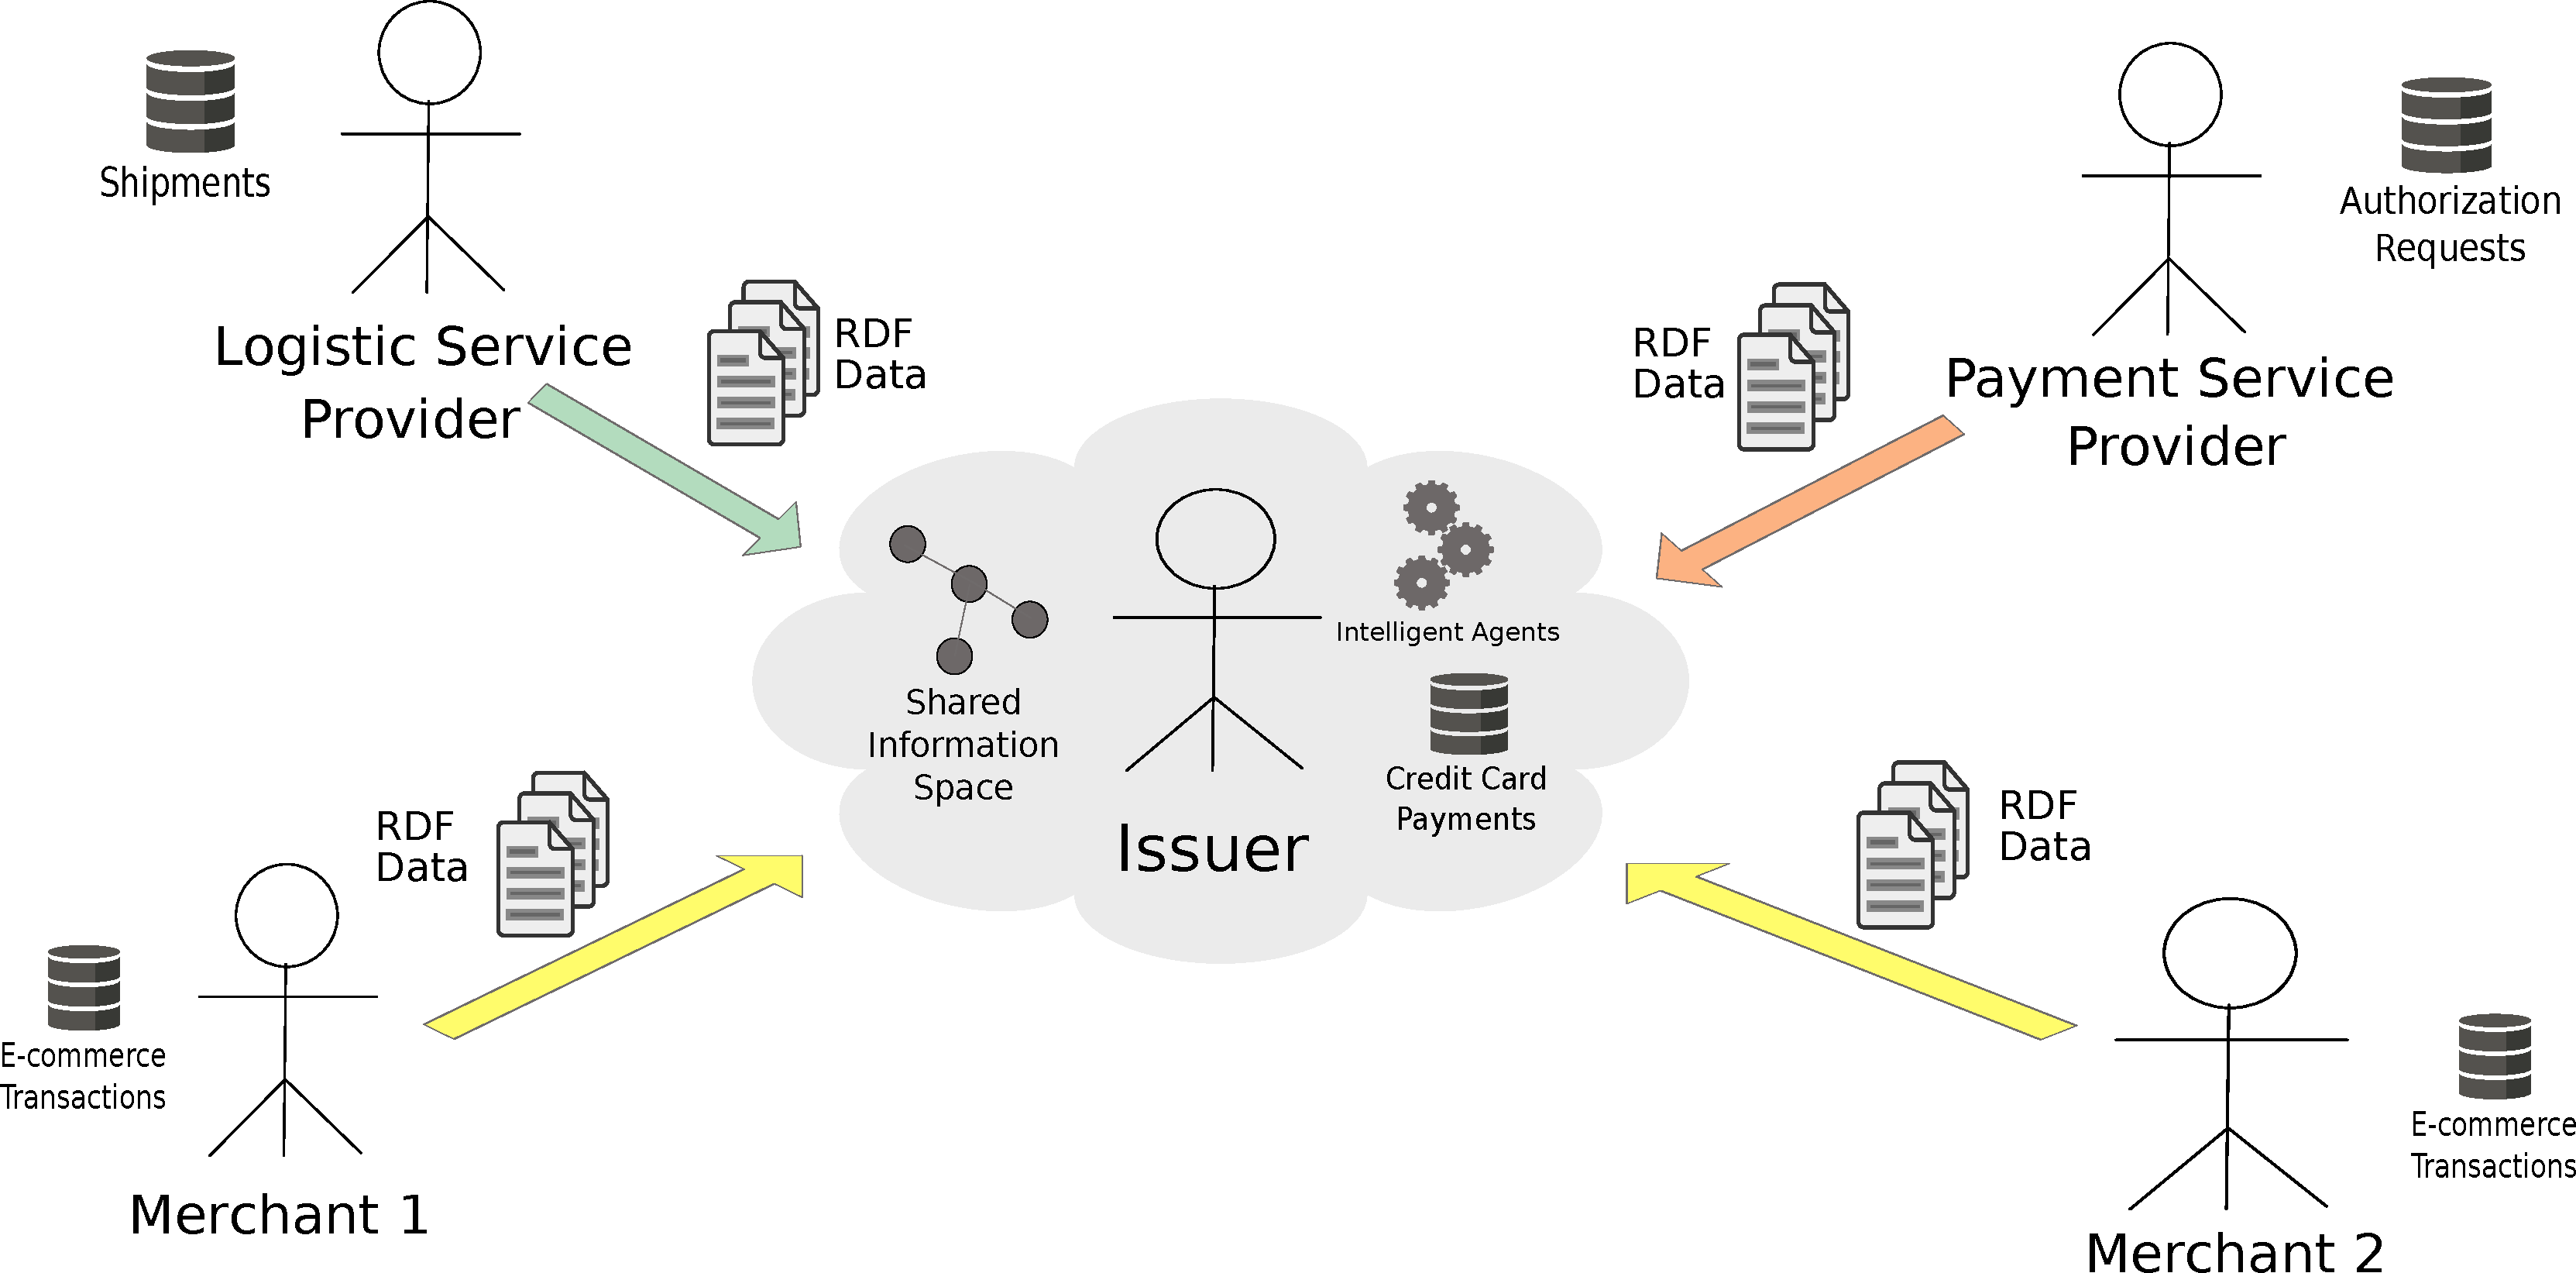
\includegraphics[width=0.9\columnwidth]{images/system_P2P_centralized.pdf}
	\caption{Collaborative system using a partially centralized \gls{P2P} architecture}
\label{fig:images_p2p_centralized}
\end{figure}

Using the \gls{WebRTC} communication protocol for initiating the \gls{P2P} session will allow the issuers to setup a communication between the relevant stakeholders directly from within an application running in their Web browsers. The application can visualize the connectivity status of the participants, the progress of their data sharing efforts as well as offer direct face-to-face communication possibilities in case of misunderstandings or further requests. A wireframe of the Web application screen is depicted in Figure~\ref{fig:images_p2p_initial_screen}. \@

\begin{figure}[H]
	\centering
		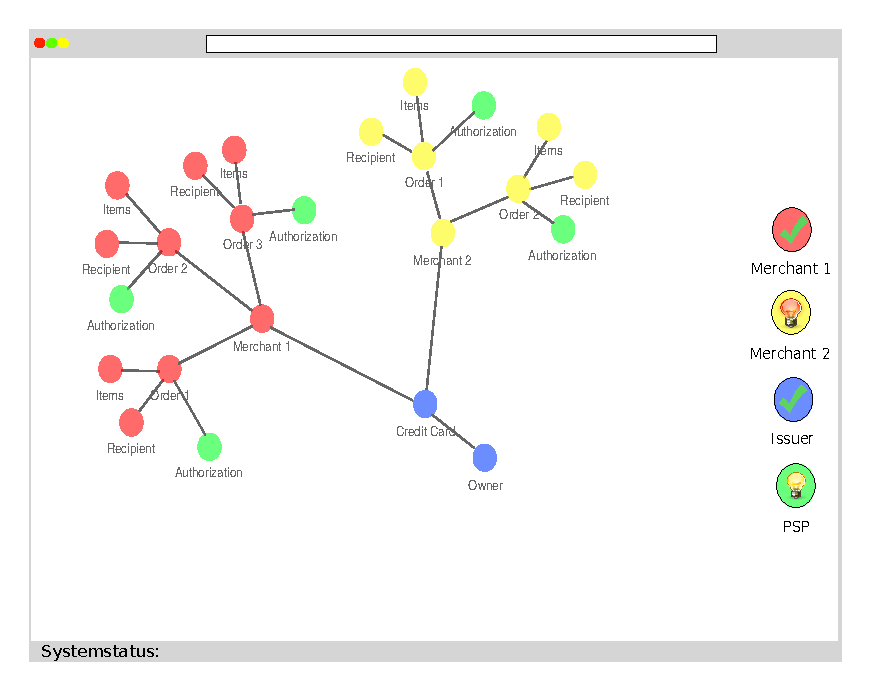
\includegraphics[width=0.9\columnwidth]{images/p2p_initial_screen.pdf}
	\caption{Screen prototype of collaborative system showing participants and shared information}
\label{fig:images_p2p_initial_screen}
\end{figure}

Main issue with the above mentioned system architecture is, that the merchants, payment and logistic service providers have to hand over their information to the issuing bank of the credit card for analysis. This might be either problematic due to distrust of the objectives of the issuing bank, or not possible at all due to local data sharing restrictions and regulations.

% subsec p2p_partially_centralized_system

% section design_proposal (end)


% chapter design system (end)
